\documentclass[tikz,border=5pt]{standalone}
\usepackage[UTF8]{ctex}
\usepackage{amsmath,amssymb}
\usetikzlibrary{arrows.meta,calc,angles,quotes,decorations.pathmorphing}
\definecolor{ink}{HTML}{243447}\definecolor{blue}{HTML}{2765A2}
\definecolor{green}{HTML}{3F7D5B}\definecolor{red}{HTML}{B74739}
\tikzset{body/.style={draw=ink,thick},vec/.style={draw=blue,thick,-{Latex}},guide/.style={gray!65,dashed},dim/.style={ink,{Latex}-{Latex}},line cap=round,line join=round}
\begin{document}
\begin{tikzpicture}
\begin{scope}
\draw[vec](-.35,0)--(3.3,0)node[right]{$x$};
\draw[vec](0,-.3)--(0,2.2)node[above]{$y$};
\fill[ink](0,0)circle(.06)node[below left]{$M$};
\fill[ink](2.3,0)circle(.06)node[below]{$m$};
\draw[vec](2.3,.1)--(2.3,1.3)node[right]{$v_0$};
\draw[dim](0,-.65)--(2.3,-.65)node[midway,below]{$r_0$};
\node at(1.4,-1.4){（a）};
\end{scope}
\begin{scope}[shift={(6.3,0)}]
\draw[vec](-1.35,0)--(3.5,0)node[right]{$x$};
\draw[vec](0,-.3)--(0,2.8)node[above]{$y$};
\fill[ink](-1,0)circle(.06)node[below]{$3m\,(-r_0,0)$};
\fill[ink](3,0)circle(.06)node[below]{$m\,(3r_0,0)$};
\fill[ink](0,1.732)circle(.06)node[left]{$2m$};
\node[right]at(.1,1.55){$(0,\sqrt3r_0)$};
\draw[vec](0,1.82)--(0,2.5)node[right]{$v_0$};
\node at(1,-1.4){（b）};
\end{scope}
\end{tikzpicture}
\begin{tikzpicture}
\begin{scope}
\draw[vec](-2,0)--(2.15,0)node[right]{$x$};
\draw[vec](0,-1.2)--(0,1.5)node[above]{$y$};
\draw[blue,thick](0,0)ellipse(1.6 and 1);
\fill[ink](0,0)circle(.055)node[below left]{$M$};
\fill[green](1.6,0)circle(.055)node[below right]{$m$};
\node at(0,-1.8){$r_0$ 与 $v_0/\omega_1$ 为半轴};
\end{scope}
\begin{scope}[shift={(6,0)}]
\coordinate(C)at(0,0);\coordinate(A)at(-.7,-.25);\coordinate(B)at(1.4,.5);
\draw[body](A)--(B);
\fill[ink](A)circle(.07)node[below left]{$2m$};
\fill[ink](B)circle(.05)node[right]{$m$};
\fill[red](C)circle(.045)node[below]{$C$};
\draw[dim](-.7,.45)--(1.4,1.2)node[midway,above]{$\boldsymbol q$};
\draw[vec](0,.1)--(0,1.3)node[left]{$v_0/3$};
\node at(.3,-1.4){$\boldsymbol r_m=\boldsymbol C+\frac23\boldsymbol q$};
\end{scope}
\end{tikzpicture}
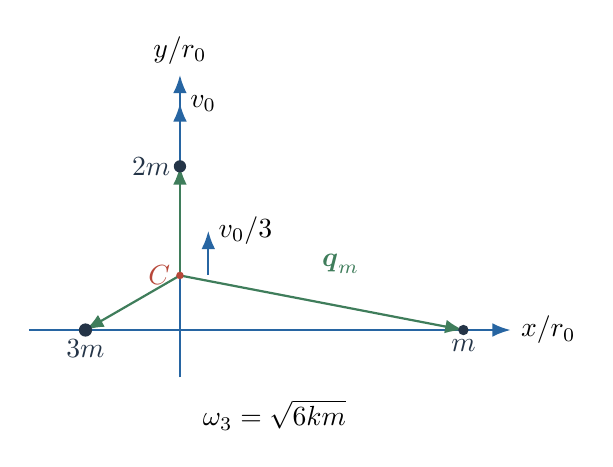
\begin{tikzpicture}[scale=1.2]
\draw[vec](-1.6,0)--(3.5,0)node[right]{$x/r_0$};
\draw[vec](0,-.5)--(0,2.7)node[above]{$y/r_0$};
\coordinate(C)at(0,.57735);
\draw[green,thick,-{Latex}](C)--(3,0);
\draw[green,thick,-{Latex}](C)--(-1,0);
\draw[green,thick,-{Latex}](C)--(0,1.732);
\fill[red](C)circle(.04)node[left]{$C$};
\fill[ink](3,0)circle(.055)node[below]{$m$};
\fill[ink](-1,0)circle(.07)node[below]{$3m$};
\fill[ink](0,1.732)circle(.065)node[left]{$2m$};
\draw[vec](0,1.83)--(0,2.4)node[right]{$v_0$};
\draw[vec](.3,.58)--(.3,1.05)node[right]{$v_0/3$};
\node[green]at(1.7,.7){$\boldsymbol q_m$};
\node at(1,-.9){$\omega_3=\sqrt{6km}$};
\end{tikzpicture}
\begin{tikzpicture}[x={(.95cm,-.12cm)},y={(.5cm,.35cm)},z={(0cm,1cm)}]
\fill[blue!5](-2,-2,0)--(2,-2,0)--(2,2,0)--(-2,2,0)--cycle;
\draw[body](-2,-2,0)--(2,-2,0)--(2,2,0)--(-2,2,0)--cycle;
\draw[vec](0,0,0)--(0,0,2.3)node[above]{$z$};
\fill[red](0,0,0)circle[radius=1.8pt]node[below]{$C$};
\fill[ink](-.65,0,0)circle[radius=2.2pt]node[below left]{$2m$};
\fill[ink](1.3,0,0)circle[radius=1.8pt]node[below right]{$m$};
\draw[body,dashed](-.65,0,0)--(1.3,0,0);
\fill[green](.7,.8,0)circle[radius=1.8pt]node[right]{$P$};
\fill[green](.7,.8,1.5)circle[radius=1.8pt]node[right]{$Q$};
\draw[guide](.7,.8,0)--(.7,.8,1.5);
\draw[red,thick,-{Latex}](.7,.8,1.5)--(.7,.8,.65)node[midway,right]{$a_z$};
\draw[vec](.7,.8,1.5)--(.2,.23,1.5);
\node[below,yshift=-8pt]at(current bounding box.south){平衡集合：$z=0$；质量以 $2m,m$ 示意};
\end{tikzpicture}
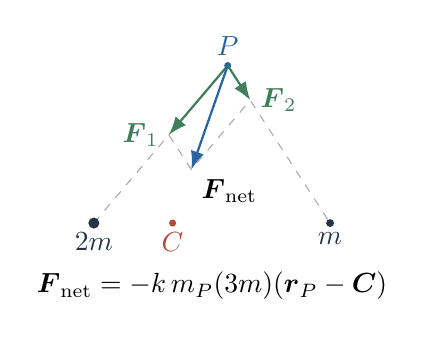
\begin{tikzpicture}
\coordinate(P)at(.7,2);\coordinate(A)at(-1,0);\coordinate(B)at(2,0);
\draw[guide](A)--(P)--(B);
\fill[ink](A)circle(.07)node[below]{$2m$};
\fill[ink](B)circle(.05)node[below]{$m$};
\fill[red](0,0)circle(.045)node[below]{$C$};
\fill[blue](P)circle(.045)node[above]{$P$};
\draw[green,thick,-{Latex}](P)--(-.048,1.12)node[left]{$\boldsymbol F_1$};
\draw[green,thick,-{Latex}](P)--(.986,1.56)node[right]{$\boldsymbol F_2$};
\draw[vec](P)--(.238,.68)node[below right]{$\boldsymbol F_{\mathrm{net}}$};
\draw[guide](-.048,1.12)--(.238,.68)--(.986,1.56);
\node at(.5,-.8){$\boldsymbol F_{\mathrm{net}}=-k\,m_P(3m)(\boldsymbol r_P-\boldsymbol C)$};
\end{tikzpicture}
\end{document}
